%*******************************************************************************
%*********************************** First Chapter *****************************
%*******************************************************************************


\chapter{Literature Survey}  %Title of the First Chapter


\graphicspath{{Chapter1/Figs/}}


%********************************** %First Section  **************************************

\section{LHCb and VELO} %Section - 1.1 

\begin{figure}[h] % h for here in document
\centering
\begin{subfigure}[t]{0.45\textwidth}
\centering
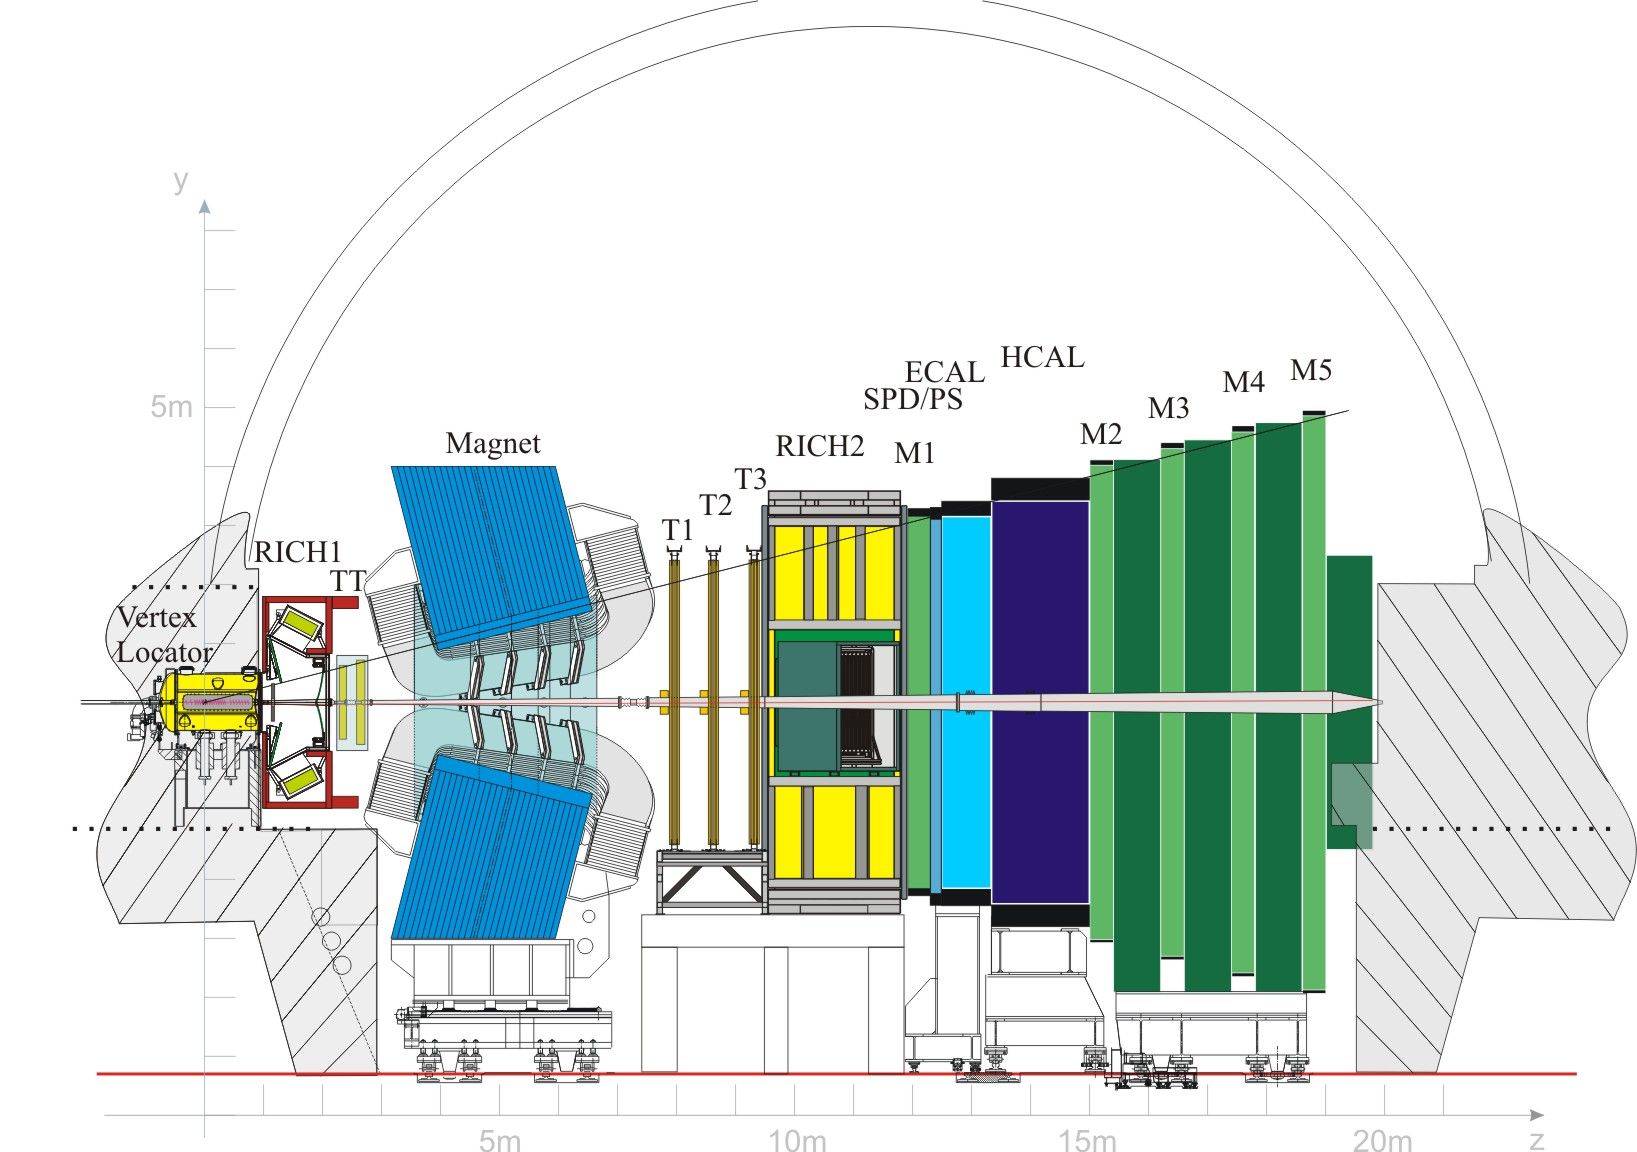
\includegraphics[width=\textwidth]{LHCbDiagram}
\caption{Diagram of LHCb detector, the VELO is on the far left. More tracking modules and calorimeters make up the detector.} 
\label{fig:LHCbDiagram} 
\end{subfigure}
~
\begin{subfigure}[t]{0.45\textwidth}
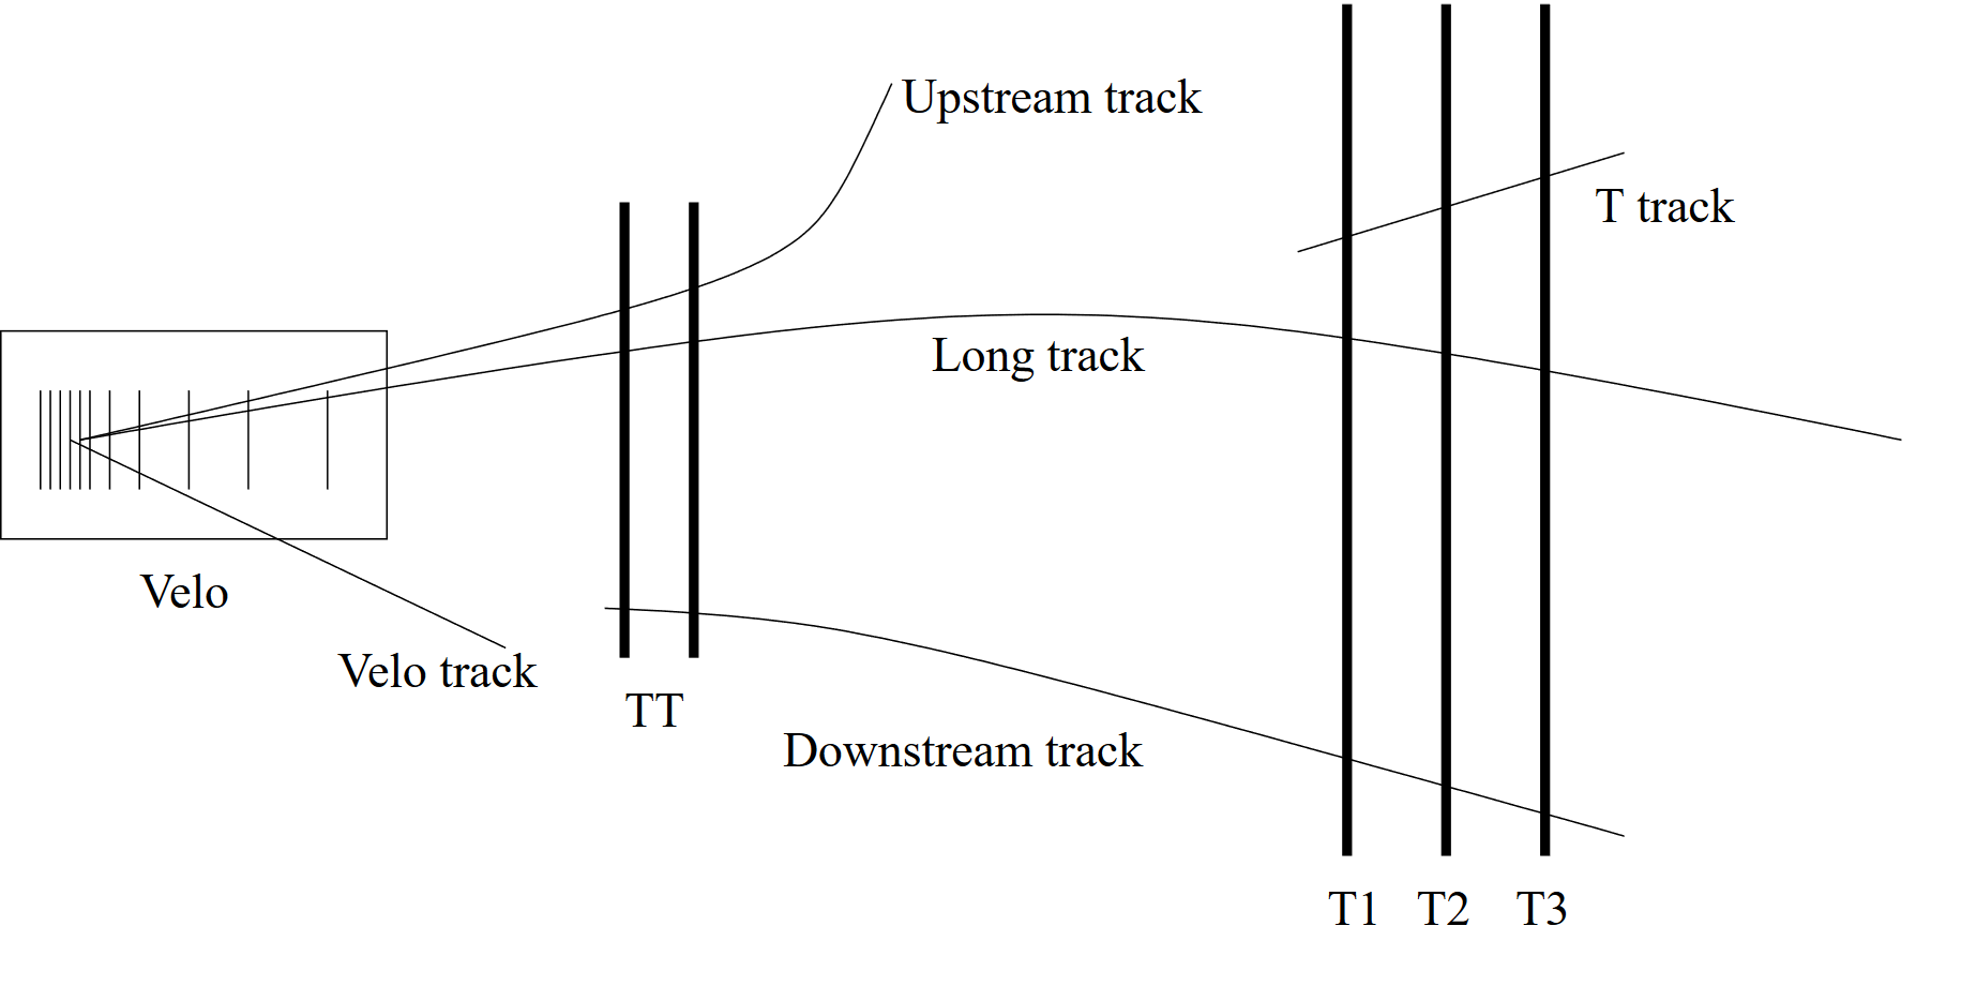
\includegraphics[width=\textwidth]{LHCbTracking}
\caption{Types of tracks found by LHCb} 
\label{fig:LHCbTracking}
\end{subfigure}
\end{figure}

\begin{figure}[h] % h for here in document
\centering
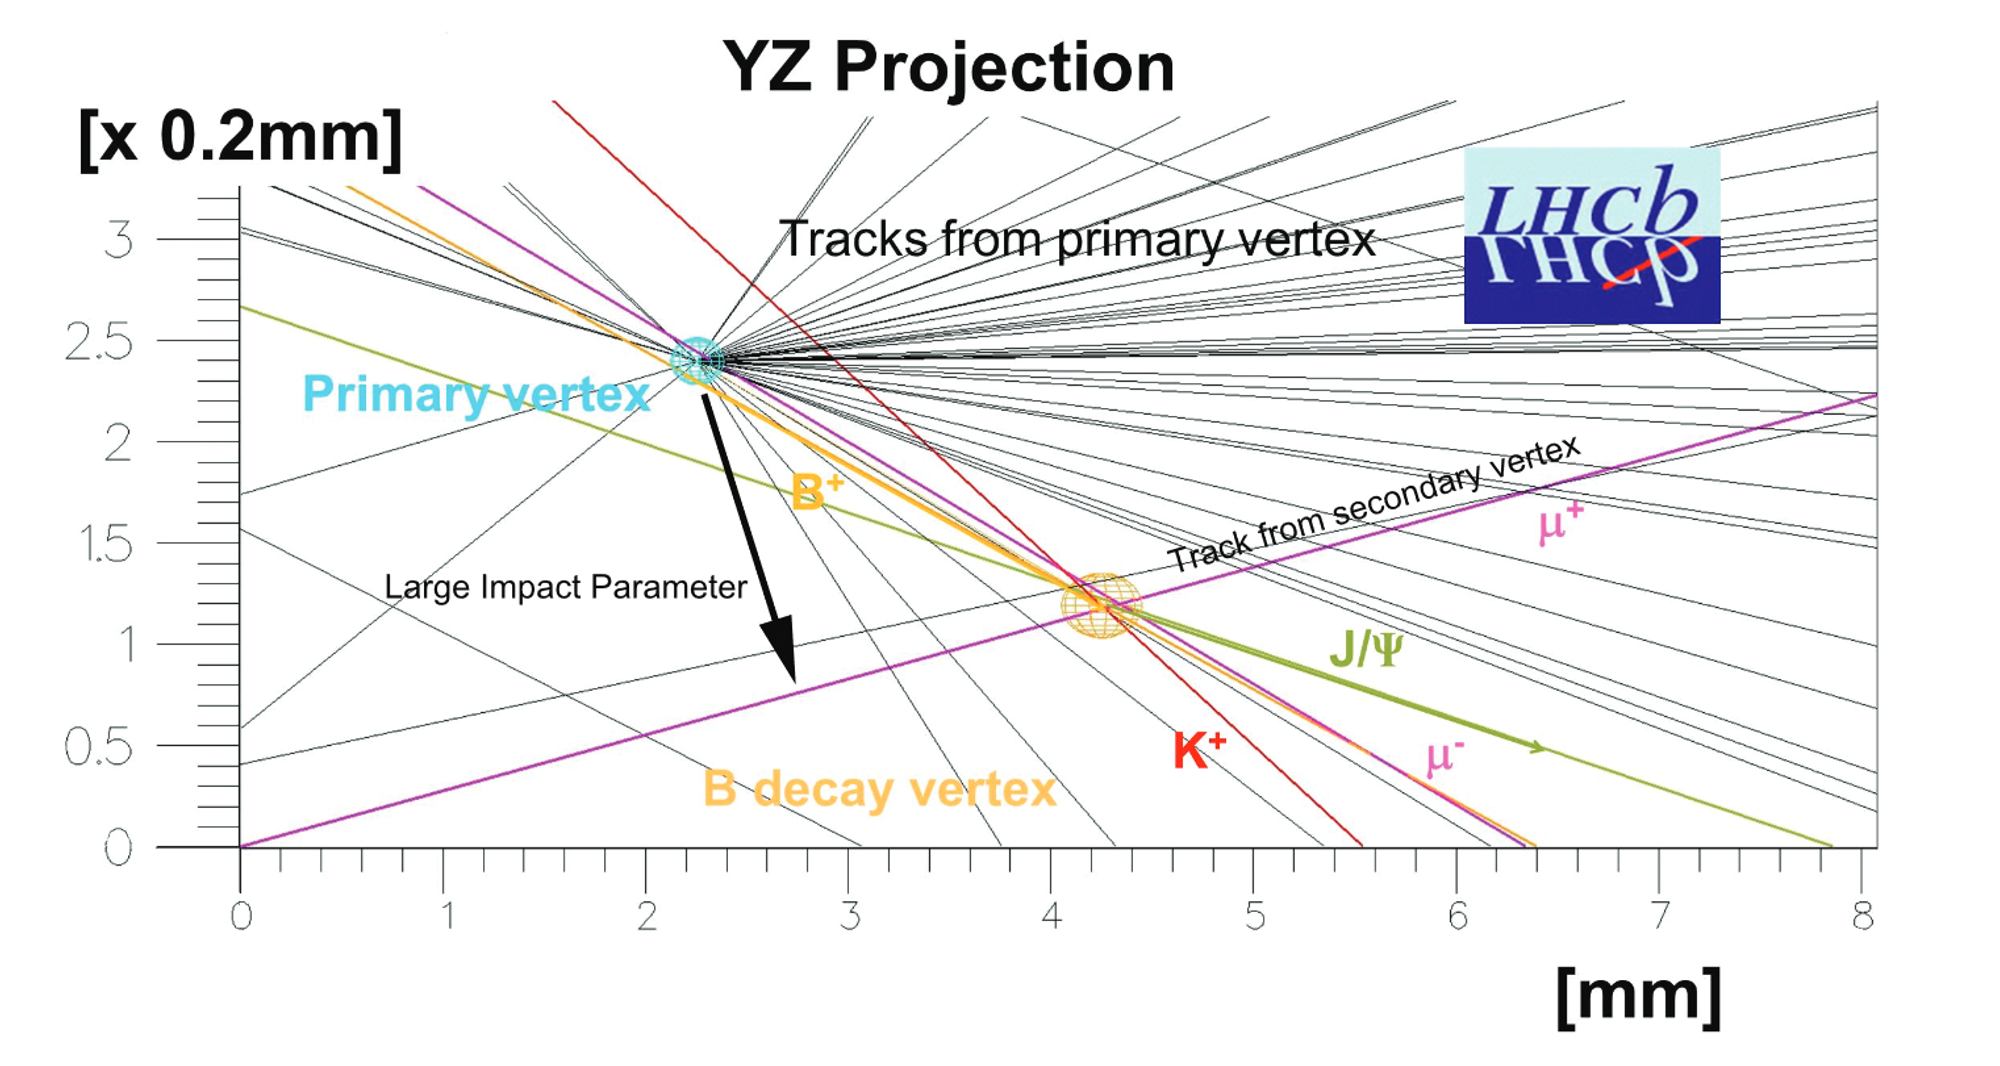
\includegraphics[width=\textwidth]{EventDiagram.png}
\caption{Diagram of typical LHCb event.} 
\label{fig:EventDiagram} 
\end{figure}

LHCb is a single-arm forward spectrometer at the Large Hadron Collider. It is designed to study heavy flavour physics and covers a pseudorapidity range of $2 < \eta < 5$. It has pioneered the search for CP violation, as well as Electroweak physics in forward direction. The experiment was designed for indirect searches of new particles, enhancing rare decay branching fractions and for precise measurements of standard model parameters \citep{Collaboration2008TheLHC}. The design of LHCb is shown in figure \ref{fig:LHCbDiagram}. Unlike other LHC experiments LHCb does not look in all directions around the collision point, instead it looks in the forward region only, with the collision point at one end of the experiment. At this collision point is positioned the Vertex Locator (VELO). Vertex location is fundamental to the success of LHCb \citep{Barbosa-Marinho:504321}. A vertex is the point in space that particles are created or decay. b-meson decays, which LHCb searches for, have distinctive displaced secondary vertices which must be correctly identified to determine decay lifetimes and tag flavours of particles. The primary vertex is the point of the first collision, at the LHC this is the proton-proton (pp) collision. A secondary vertex is the point of decay of products of the first decay. b-meson decays are identified by their impact parameter (IP), the distance between the primary vertex and the nearest point on the track \cite{Kucharczyk:1756296} see figure \ref{fig:LHCbTracking}. Primary vertices are found from tracks reconstructed by the VELO. A track is a series of connected hits in the detector that were created by the same particle, correctly reconstructing tracks from hits in the detector can be used to identify particle momenta as well as finding Primary Vertices. Types of tracks found by LHCb are shown in figure \ref{LHCbTracking} \cite{LHCb2012TrackingLHCb}. Reconstructing tracks in the VELO is the primary aim of this project. Pattern recognition is the method used to identify which hits were caused by each particle, and correctly group them into tracks.

%********************************** % Second Section  *************************************

\section{LHCb and VELO Upgrade}  %Section - 1.2

The current VELO has been in operation since the start of LHC operation in 2008, however as part of the LHCb upgrade a new VELO is being constructed. The LHCb upgrade is scheduled for run-III in 2021 \cite{Hennessy2016LHCbUpgrade} and involves upgrades to many parts of the experiment. 
% Write something about what LHCb wants to measure in the future
The headline feature of the LHCb upgrade is the 5 times increase of luminosity to \(2\times10^{33} cm^{-2} s^{-1}\), this increase will require to the removal of the L0 hardware trigger, this will increase event rate from the current 1MHz to the full 40MHz event rate capable at the \cite{LHCCollaboration:1624070}. The current software triggers will also be replaced. These changes will result in more events occurring in the experiment, and more information about these events being read. For the VELO this will mean higher pile-up per event and more events per second, it can be seen therefore that the speed of pattern recognition algorithms must be greatly increased to cope.
The current VELO is a silicon strip detector consisting of 42 modules positioned around the LHCb interaction point over a range of approximately 1m shown in figure \ref{fig:CurrentVelo}. Each module contains silicon strip sensors and is split in half so that the detector can be retracted during beam injection. This is required because the VELO sensors are designed to be positioned millimetres from the beam line, during beam injection the beam is not perfectly centred, and could cause damage to the sensors. 
The upgraded VELO has a similar basic design but with many important differences figure \ref{fig:UpgradeVELO}. The number of modules will be increased to 52, and importantly the silicon strip sensors are being changed to pixel sensors. These sensors will be placed closer to the beam, just 5.1mm away compared to 8.2mm of the current VELO. Finally the new electronics will readout the sensors at 40MHz, giving a total VELO data rate of 1.2Tb/s, greatly increased from the 150Gb/s of the current VELO \cite{Hennessy2016LHCbUpgrade}. 
A diagram of a pair of modules is shown in figure \ref{fig:VeloSensorDiagram}. The VELO pixel sensors are 2d arrays of 256x256 pixels, three sensors are placed side by side to create effective 768x256 arrays. 2 of these arrays are positioned in an L shape on each side of each module. When the pair of modules are in the closed position they form an almost square array of pixel sensors \cite{Bird:1620453}. In reality these are rotated by 45 degrees.

\subsection{Motivation}
The LHCb upgrade will see a vast increase in data rate. If current computing systems are kept in place for Run III then storage capacity and computing power requirements, and to generate and reconstruct simulated events will exceed current capacity by an order of magnitude\cite{Bozzi:2298181}. However it will not be as simple as increasing computing capacity to cope as this is not likely to be funded. Therefore work must be done to ensure upgrade software is more efficient. Trigger performance was improved for Run II by means of a second High Level Trigger (HLT2), allowing physics analysis to be done directly from objects directly out of the trigger. Event data size has also been reduced using the \verb|Turbo| stream, which stores only some information about events.\\
Further performance gains can be achieved by maximising the use of parallel computing on multi-core systems and GPU's. This will involve major changes to software to utilise these benefits.


\begin{figure}[!h] % h for here in document
\centering
\begin{subfigure}[t]{0.45\textwidth}
\centering
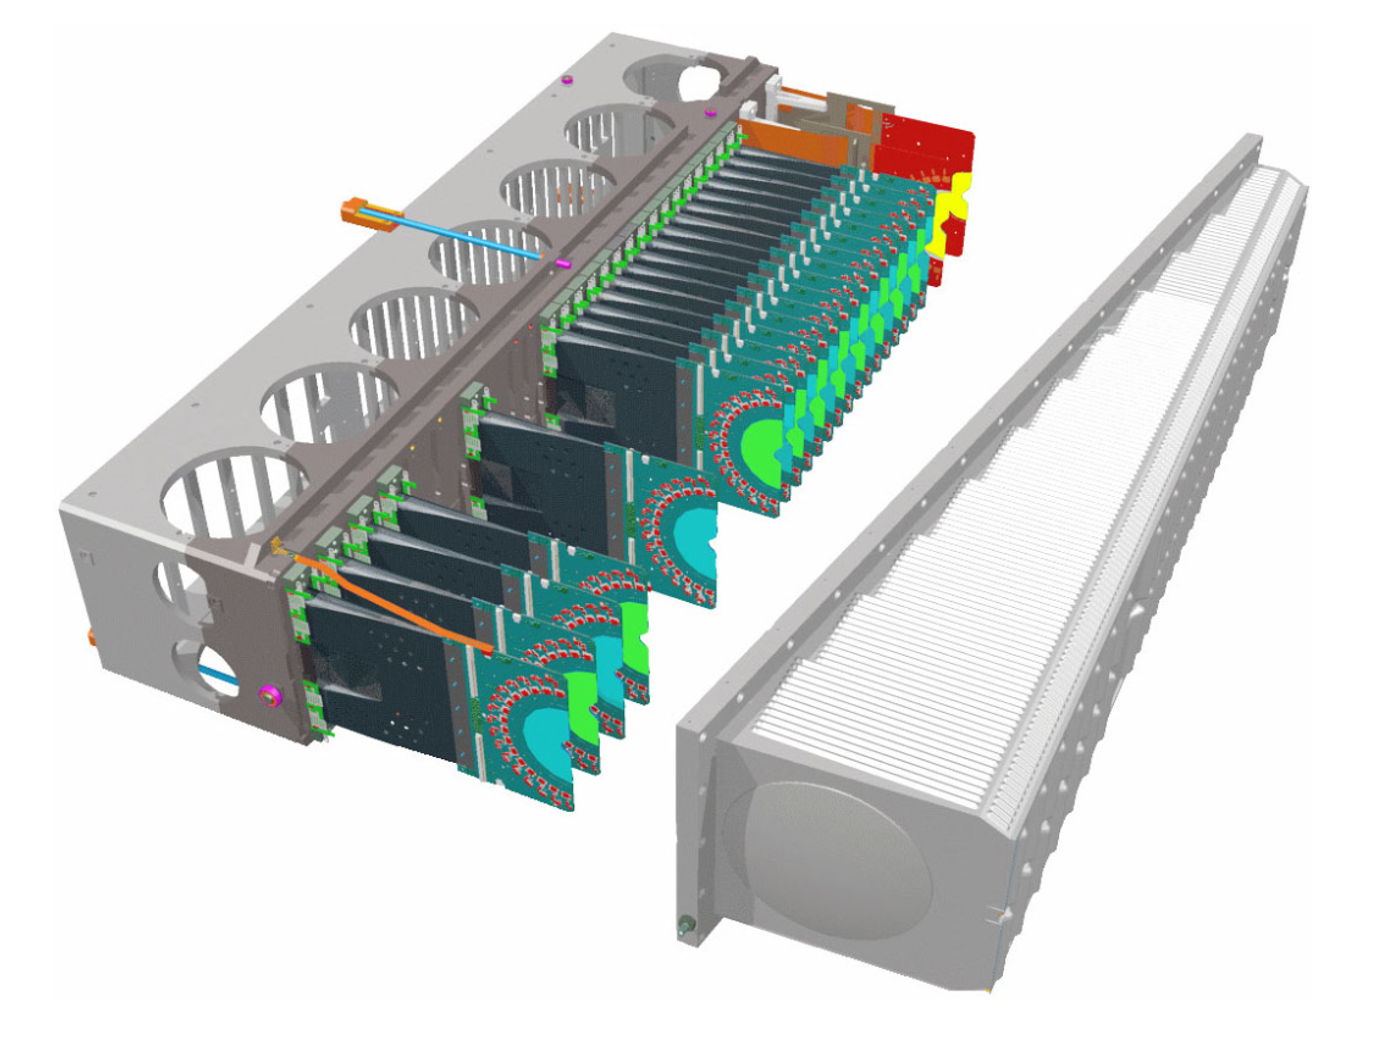
\includegraphics[width=\textwidth]{CurrentVelo}
\caption{Diagram of current VELO.} 
\label{fig:CurrentVelo} 
\end{subfigure}
~
\begin{subfigure}[t]{0.45\textwidth}
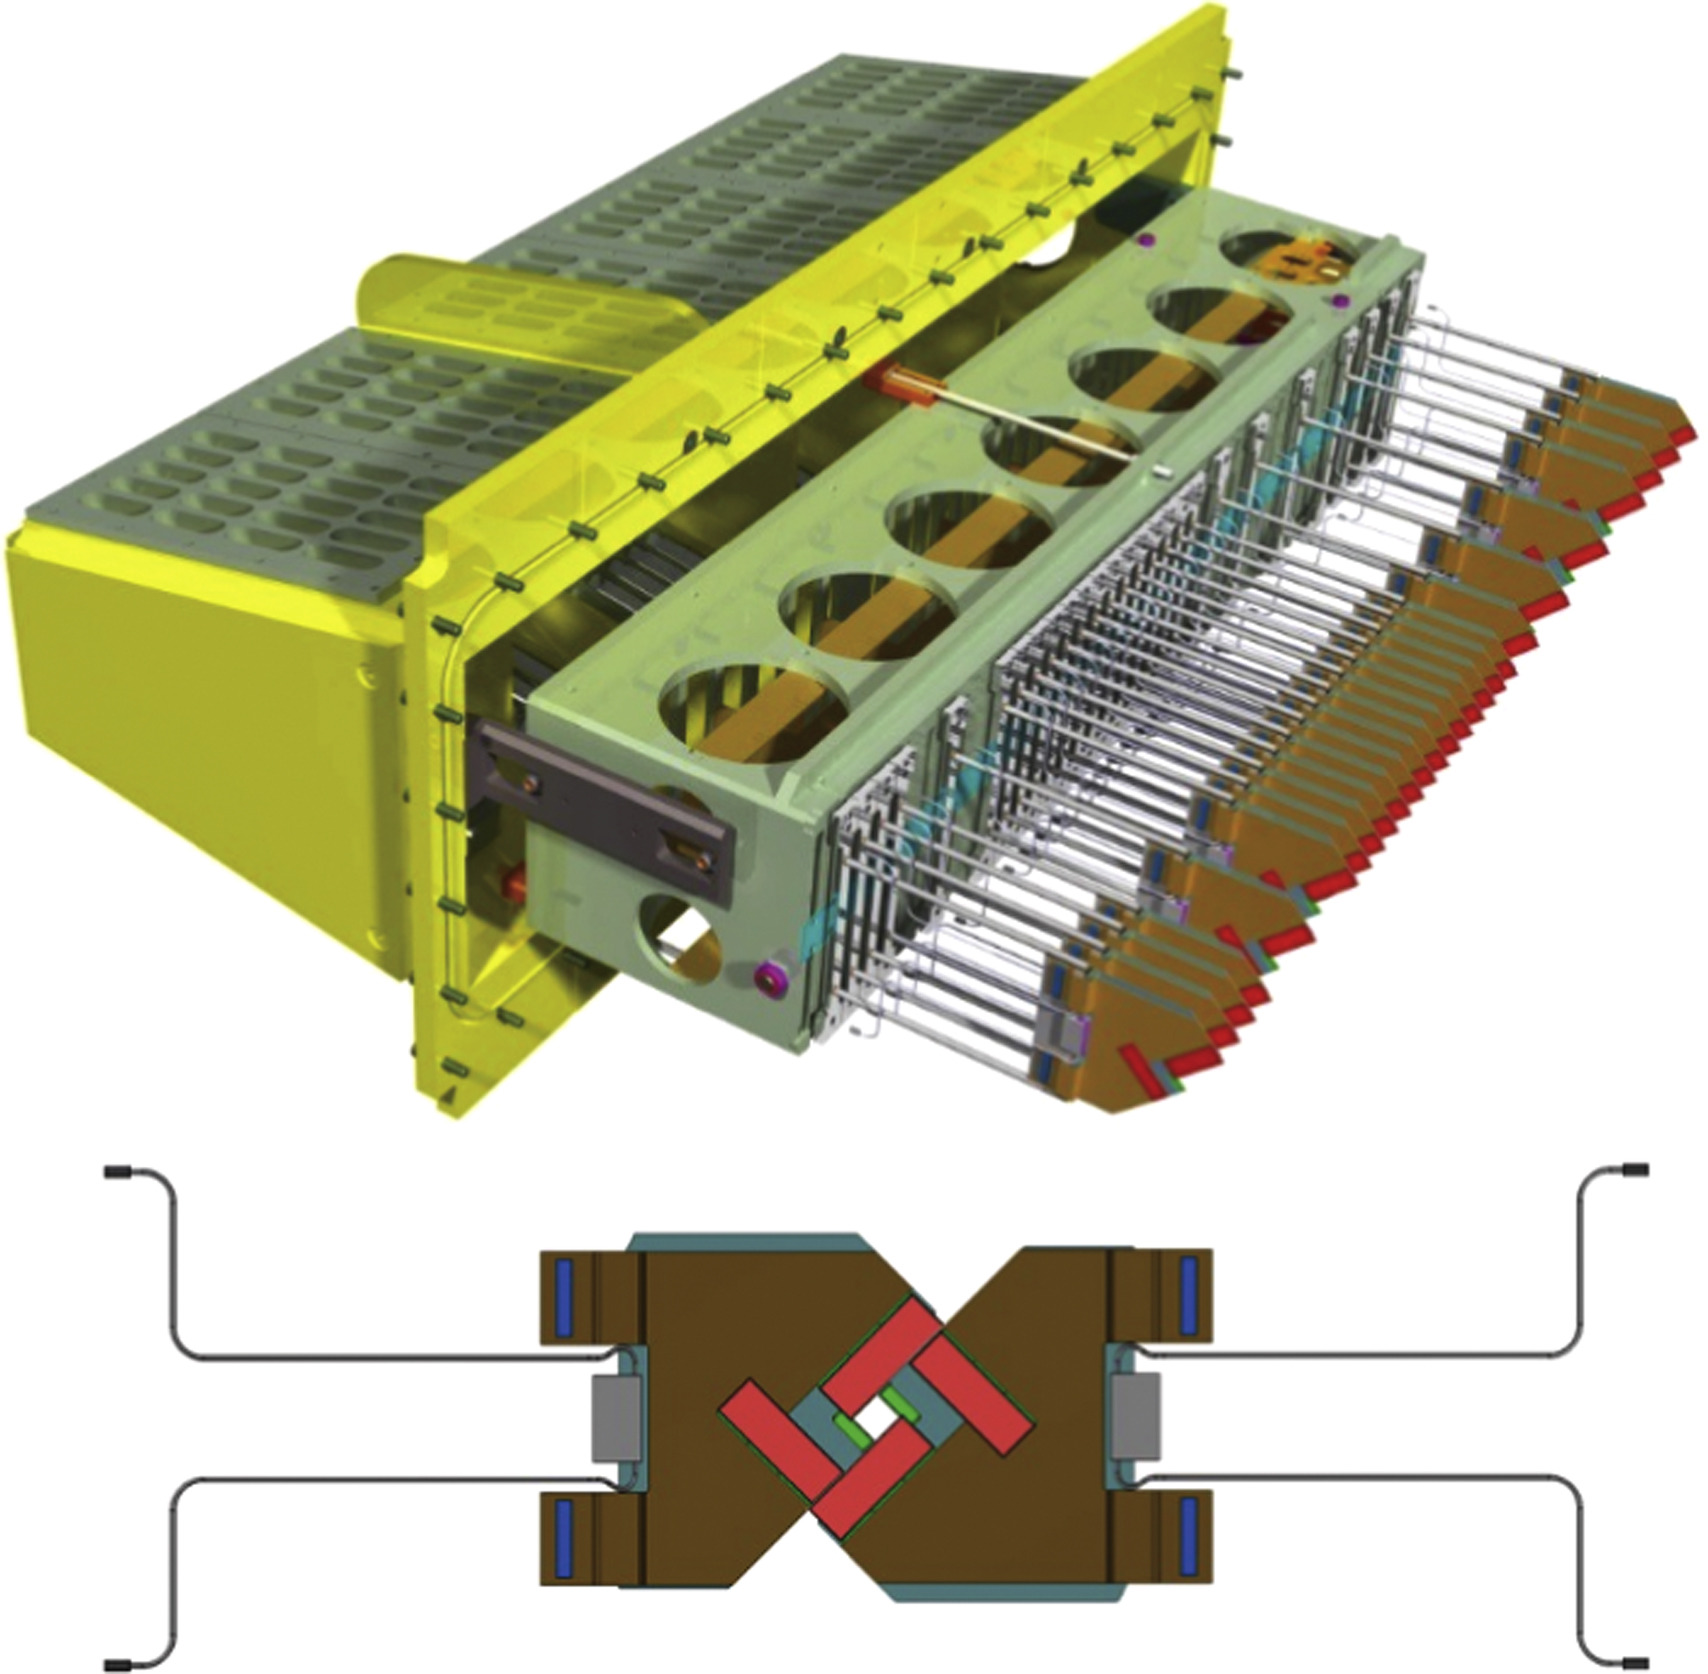
\includegraphics[width=\textwidth]{UpgradeVELO}
\caption{Diagram of upgrade VELO.} 
\label{fig:UpgradeVELO}
\end{subfigure}
\end{figure}

\begin{figure}[!h] % h for here in document
\centering
\begin{subfigure}[t]{0.45\textwidth}
\centering
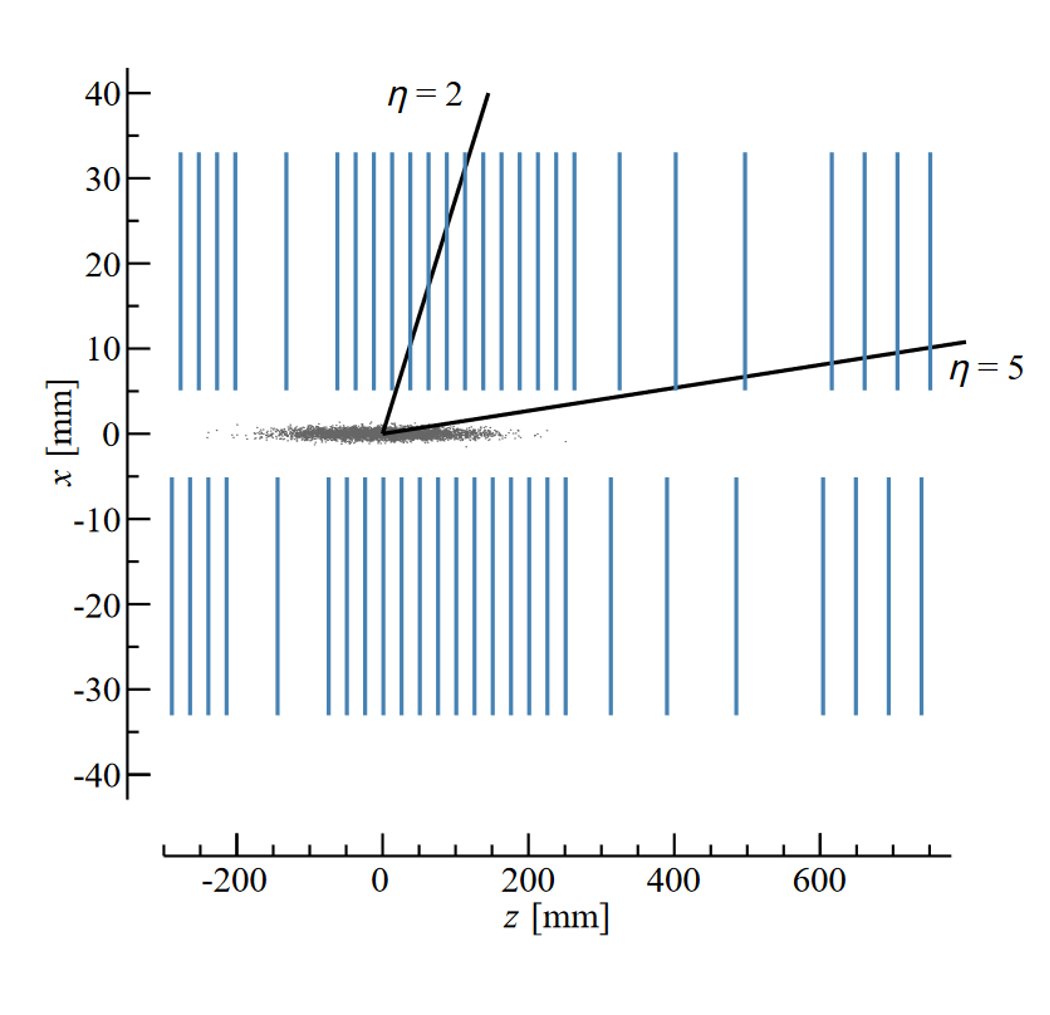
\includegraphics[width=\textwidth]{VeloLayerDiagram}
\caption{Diagram of VELO upgrade module layout.} 
\label{fig:VeloLayerDiagram} 
\end{subfigure}
~
\begin{subfigure}[t]{0.45\textwidth}
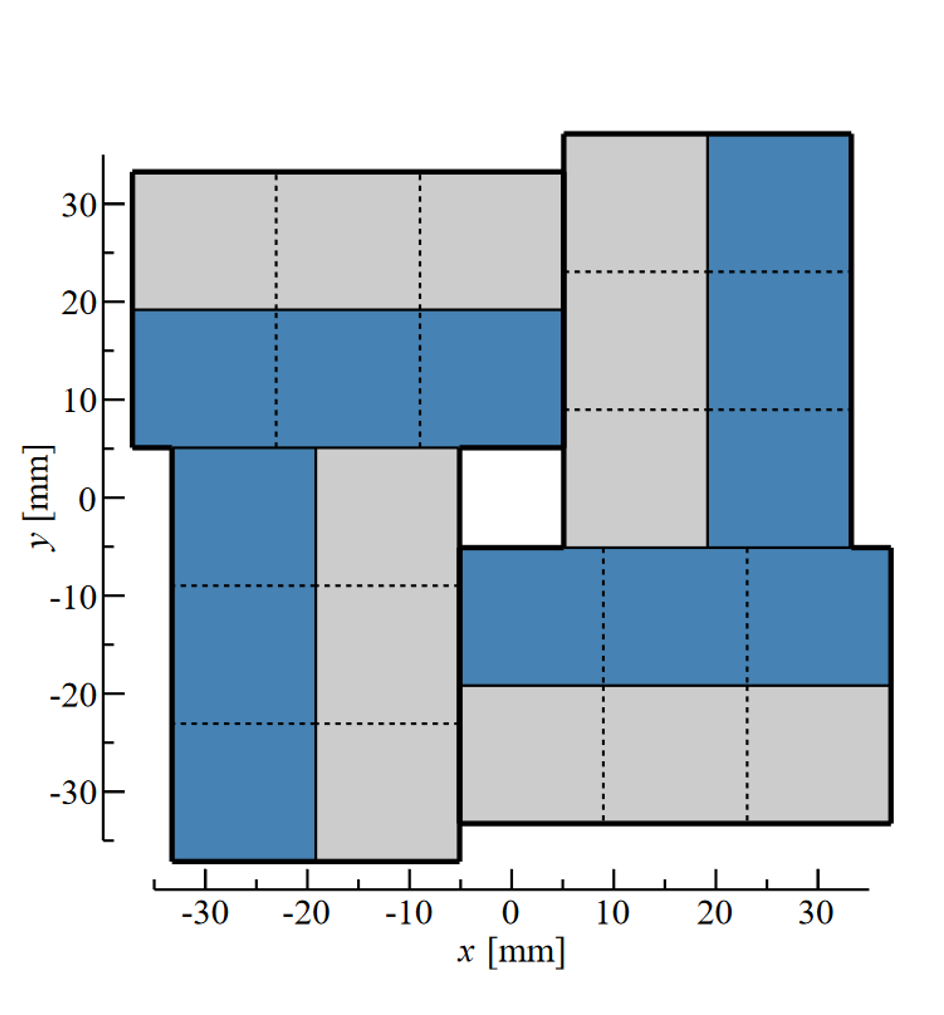
\includegraphics[width=\textwidth]{VeloSensorDiagram}
\caption{Diagram of VELO sensors on each module. Blue sensors are on one side, grey on the other side of the module.} 
\label{fig:VeloSensorDiagram}
\end{subfigure}
\end{figure}

%********************************** %Third Section  *************************************

\section{VELO Track Reconstruction} %Section - 1.3
VELO track reconstruction is the name for a series of algorithms that takes hits in the VELO and returns tracks. These tracks are then used for physics analysis. This section will describe the known method for VELO upgrade track reconstruction \cite{Bird:1620453}.

\subsection{Clustering}
Particles will often deposit energy in more than one pixel in each sensor. A group of pixels belonging to the same hit is known as a cluster. The number of pixels in a cluster is determined by the angle the particle passed through the sensor. A steeper angle will create large clusters whilst shallower angles will create smaller clusters. Each pixel has a binary readout, meaning a cluster is represented by a small group of 1's in a large array of 0's.

\subsection{Pattern Recognition}
Clusters are stored with errors $\Delta$x and $\Delta$y. These errors are used for calculating weights for the track fit later in the process, and are approximated by $\Delta x = \Delta y = p/\sqrt{12}$ where $p$ is the size of each pixel.
The method of pattern recognition currently developed works as follows:
\begin{enumerate}
    \item Starting from the most downstream module (module with the largest $z$) pairs of unused clusters in the next upstream module are investigated. These cluster pairs must have track slopes $|dx/dz|<0.4$ and $|dy/dz|<0.4$. The restriction of track slopes is used so that only tracks that lead roughly towards the interaction point are looked at.
    \item Step 1 will produce a number of possible track seeds between every pair of adjacent modules, to determine which seed is correct each track seed is extrapolated to the next upstream module. A small window is drawn around each extrapolated hit in the 3rd module, if there are any clusters inside this window then this cluster will be added to the track.
    \item After this process is complete tracks that contain less than three clusters are rejected. Tracks with exactly three clusters must contain only unused clusters and pass a cut on the track $\chi^2$ from a least-squares fit. Tracks with more contain more than three clusters must at least 50\% unused clusters, if this is true then all clusters are added to the track and tagged as used.
    \item The next stage is to convert each temporary track to a \verb|Track::Velo| object. If the z-position at which the track is closest to the beam line is larger than the maximum z-position of any cluster then the track is labelled as a backward track, otherwise it is labelled as a forward track. The track is then fit using a Kalman filter with scattering. This method if fitting gives better impact parameter resolution than a standard straight line fit. The scattering per layer is approximated by
    $$\sigma_{MS}^{2}=a+b(t_{x}^{2}+t_{y}^{2})$$
    where $t_x$ and $t_y$ are the track slopes and $a$ and $b$ are parameters determined from Monte Carlo simulation.
    \item Finally track states are calculated for each track. A track state is simply an $x,y,z$ coordinate with errors on $x$ and $y$. Track states are calculated for each track at a z-position closest to the beam line and at the end of the VELO (defined as z=770mm).
\end{enumerate}
It is this step I will be trying to improve through the application of machine learning.

\subsection{Efficiency}
Monte Carlo simulation truth can be used to calculate the efficiency of this method. The efficiency is calculated by comparing the number of correctly reconstructed tracks to the number of reconstructible tracks from the MC. The following definitions are used by LHCb:

\begin{itemize}
    \item A track is reconstructible as a VELO track if there are clusters associated to it on three or more modules
    \item A track is reconstructible as a “long track” if it is reconstructible as a VELO track and, in addition, has at least one x and one “stereo” hit in each of the three downstream track seeding stations.
    \item A particle is considered reconstructed if at least 70\% of the measurements on a track are associated to this particle.
    \item A ghost track or fake track is a track which cannot be associated to any simulated particle.  If more than one reconstructed track is associated to a particle the extra tracks are counted as clone tracks.
    \item $\epsilon_{rec}=\frac{N_{correctly\ reconstructed}}{N_{reconstructible}}$
\end{itemize}
The method described above can achieve very high efficiency's of >99\%, more than that of the current VELO \cite{Collaboration:1624070}. However it is not optimised for speed.




%********************************** % Fourth Section  *************************************

\section{Machine Learning}  %Section - 1.4
Machine learning is not a new idea, but has seen a great increase in popularity in recent years. The history of machine learning is almost as old as computing itself, it was in 1950 that Alan Turing published \textit{Computing Machinery and Intelligence} \cite{TURING1950I.COMPUTINGINTELLIGENCE}, in which he laid out his ideas about the ability of machines to think and learn. Turing's criteria have since become known as the 'Turing Test'. Initial research into machine learning took the form of mimicking the neurons in the brain, and it was in 1957 that Frank Rosenblatt invented the \textit{perceptron}. A perceptron is an algorithm for binary linear classification see figure \ref{fig:SingleLayerPerceptron}. It can decide if an object is one of two classes and can draw a straight line to differentiate populations of objects shown in figure \ref{fig:Perceptron_example}.  

\begin{figure}[h] % h for here in document
\centering
\begin{subfigure}[t]{0.45\textwidth}
\centering
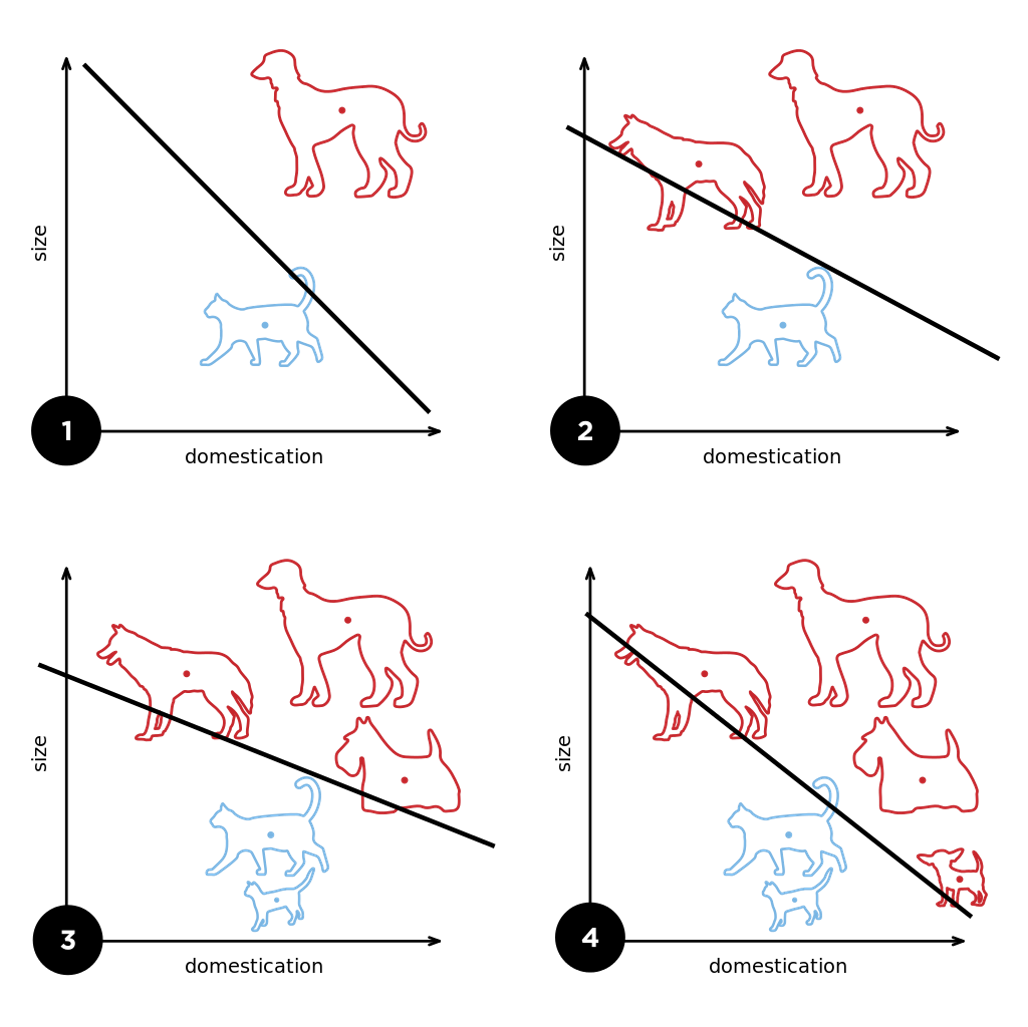
\includegraphics[width=\textwidth]{Perceptron_example}
\caption{A diagram of a perceptron learning to change its linear boundary as more training data is added. In this it is classifying whether an animal is a cat or a dog depending on its size and level of domestication.} 
\label{fig:Perceptron_example} 
\end{subfigure}
~
\begin{subfigure}[t]{0.45\textwidth}
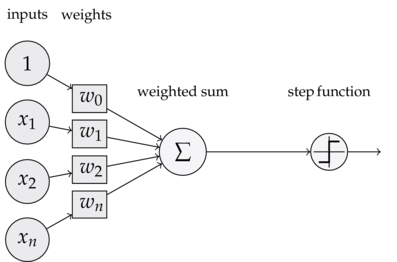
\includegraphics[width=\textwidth]{SingleLayerPerceptron}
\caption{Diagram of a single layer perceptron, as described by Rosenblatt. A feature vector is fed in and a weighted sum is made of the features. A step function is used as an activation to give the binary output of 0 or 1.} 
\label{fig:SingleLayerPerceptron}
\end{subfigure}
\end{figure}

Rosenblatt was highly optimistic about the abilities of the perceptron. However in 1969 Marvin Minsky and Seymour Papert published their book \textit{Perceptrons: an introduction to computational geometry} \cite{Minsky1969Perceptrons:Geometry} in which they proved mathematically that a single layer perceptron could not learn, for example, the XOR logic function. This controversial book signalled the start of the first 'dark age' of machine learning, however it was not to last long.\\
Machine learning research would rise again after the invention of \textit{back propagation}. Back propagation was a new method of learning developed by David Rumelhart, Geoffrey Hinton  and Ronald Williams and published in 1986 \cite{Rumelhart1986LearningErrors}. This paper introduced the idea of a network of 'hidden layers', unlike previous multilayer perceptrons these hidden layers had weights set by a back propagation algorithm, rather than by hand. The back propagation algorithms job was to tune the weights of neurons to reduce the difference between the network output and the desired output. This breakthrough allowed these 'neural networks' to learn non-linear functions, not possible with simple perceptrons. Further papers proved that neural networks could theoretically learn any non-linear function, given enough neurons \cite{Hornik1991ApproximationNetworks}. Early success was had with convolutional neural network used to identify handwritten digits \cite{LeCun1990HandwrittenNetwork}. However funding cuts, expensive systems and a long list of missed goals led an 'AI winter'. With many losing faith in artificial intelligence. This did not stop IBM, who in 1997 beat reigning world chess champion Garry Kasparov with their machine 'Deep Blue', and for the first time showed the capabilities of artificial intelligence. Deep Blue used massively parallel computing to calculate hundreds of millions of positions every second \cite{Campbell2002DeepBlue}. This brute force approach is not the same as other machine learning methods discussed.\\
It was not until the 'big data' revolution of the 21st century that machine learning was truly taken seriously. The mid 2000's saw a series of revolutionary papers that greatly improved the performance of neural networks. Greedy layerwise training was first proposed in 2006 \cite{Bengio2006GreedyNetworks}, as a way to initialise the weights of a neural network before the supervised learning stage. Random initialisation would often lead to poor final solutions. Increasing computing power meant that the power of neural network could finally be realised.


